\begin{chapter}{Additional residual plots  for the fitted emulators in \cref{Ch:ds-for-ow} \label{App:resid}}
\section{Plots of SLPEs for the wave $1$ emulator, with no mean function \label{App:resid1}}
We see in each of the following three groups of residual plots, that apart from $x_9$, the residuals appear randomly scattered. The variance of the residuals is too large, but we suspect that this is due to the structure present in the plots of SLPEs against $x_9$. Each warehouse has a pair of plots; one for the first $9$ inputs (the numbers of spares, scaled to $[0,1]$) and then the last $9$ inputs (critical percentages, scaled to $[0,1]$). Although the emulators did not directly take $x_1$ as an input, we have included it in the residual plots to verify that its exclusion is reasonable.
%wave 1, warehouse 1, no mean
\begin{figure}
  \centering
  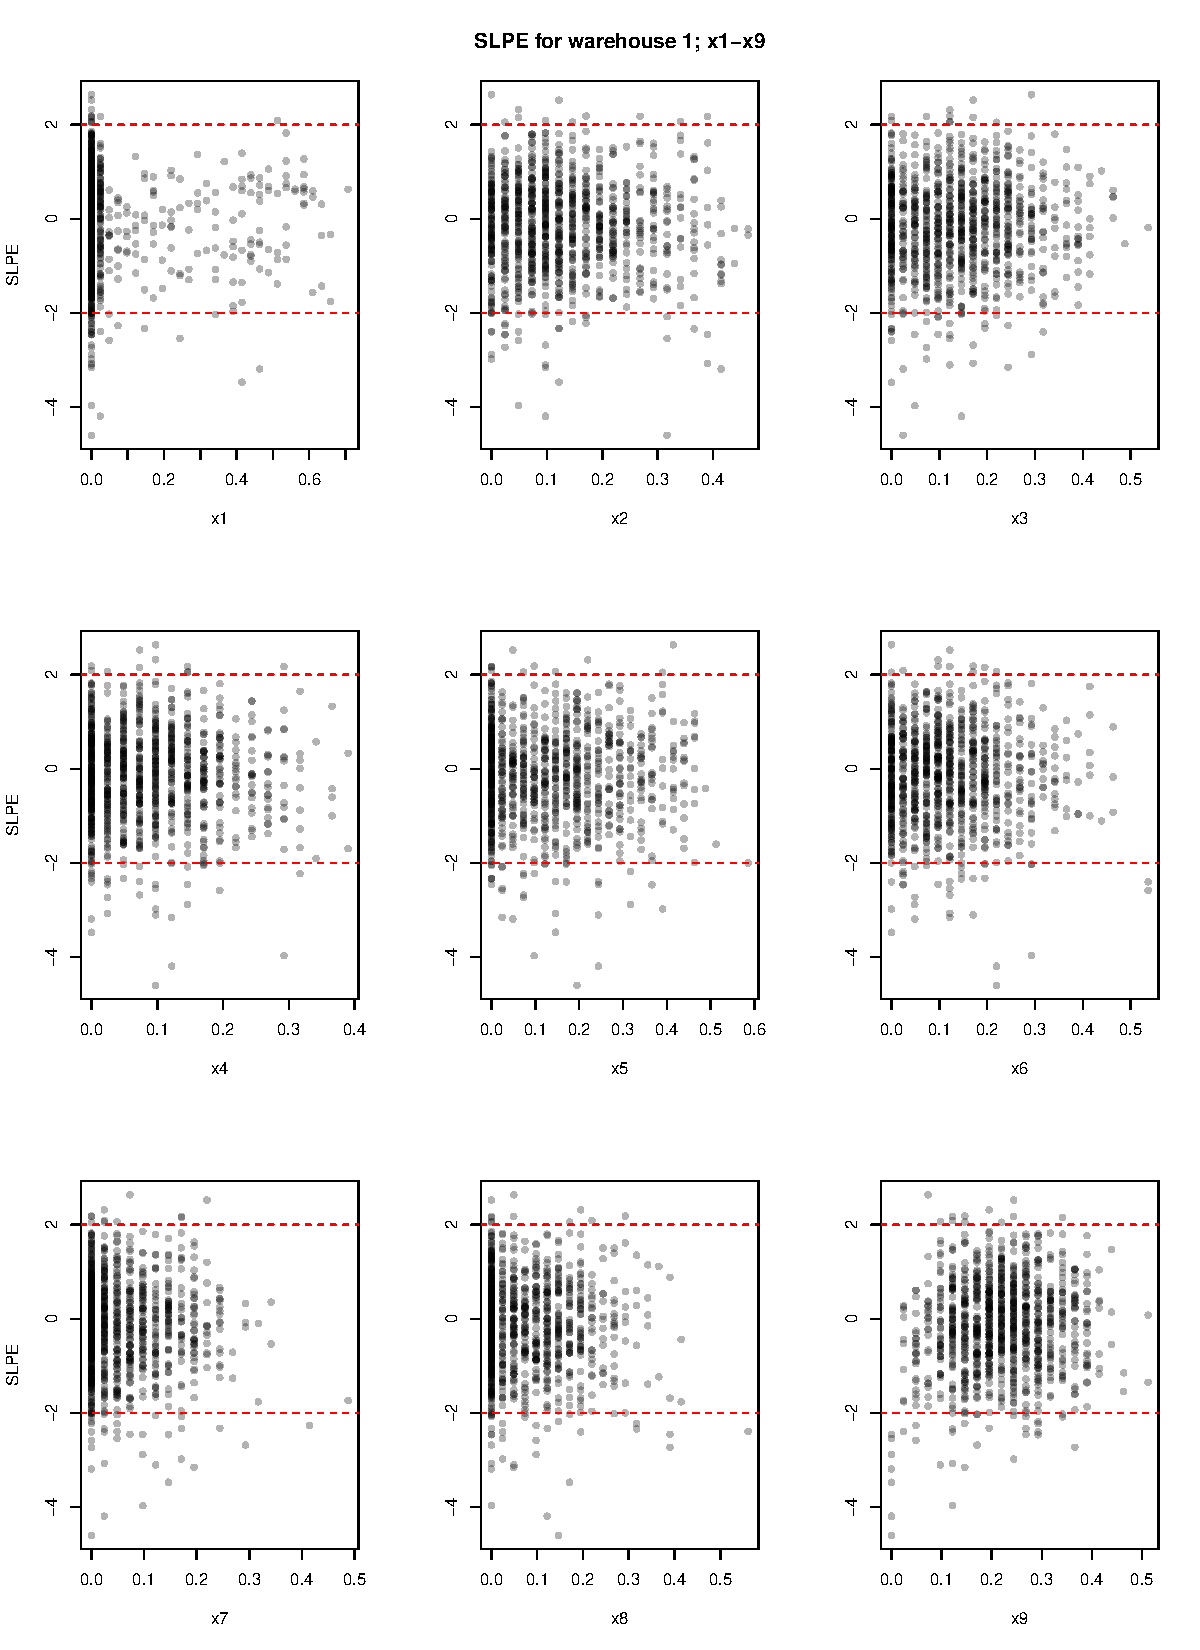
\includegraphics[width=\textwidth]{fig-app-ds/w1-w1-1.pdf}
  \caption{SLPEs for the first $9$ inputs of the wave $1$ emulator, for warehouse $1$ and $h(\bx) = 1$.}
\end{figure}

\begin{figure}
  \centering
  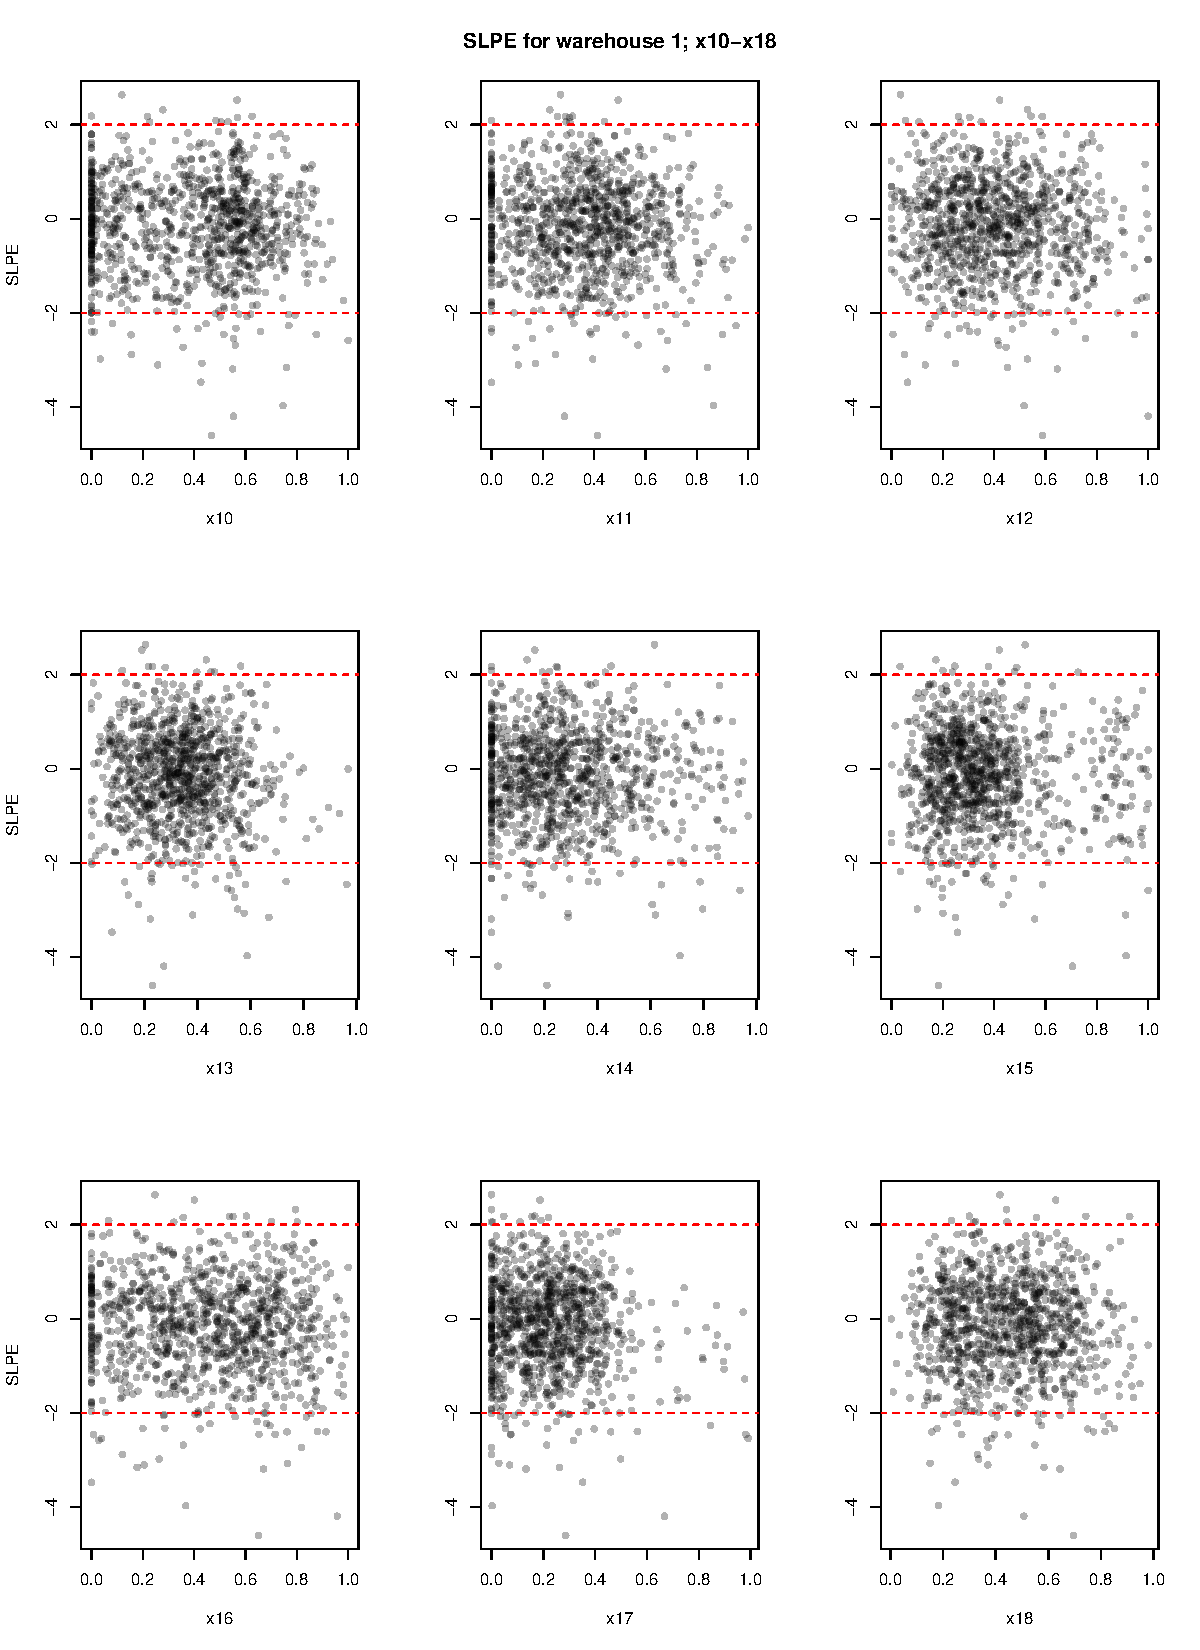
\includegraphics[width=\textwidth]{fig-app-ds/w1-w1-2.pdf}
  \caption{SLPEs for the last $9$ inputs of the wave $1$ emulator, for warehouse $1$ and $h(\bx) = 1$.}
\end{figure}
%wave 1, warehouse 2, no mean
\begin{figure}
  \centering
  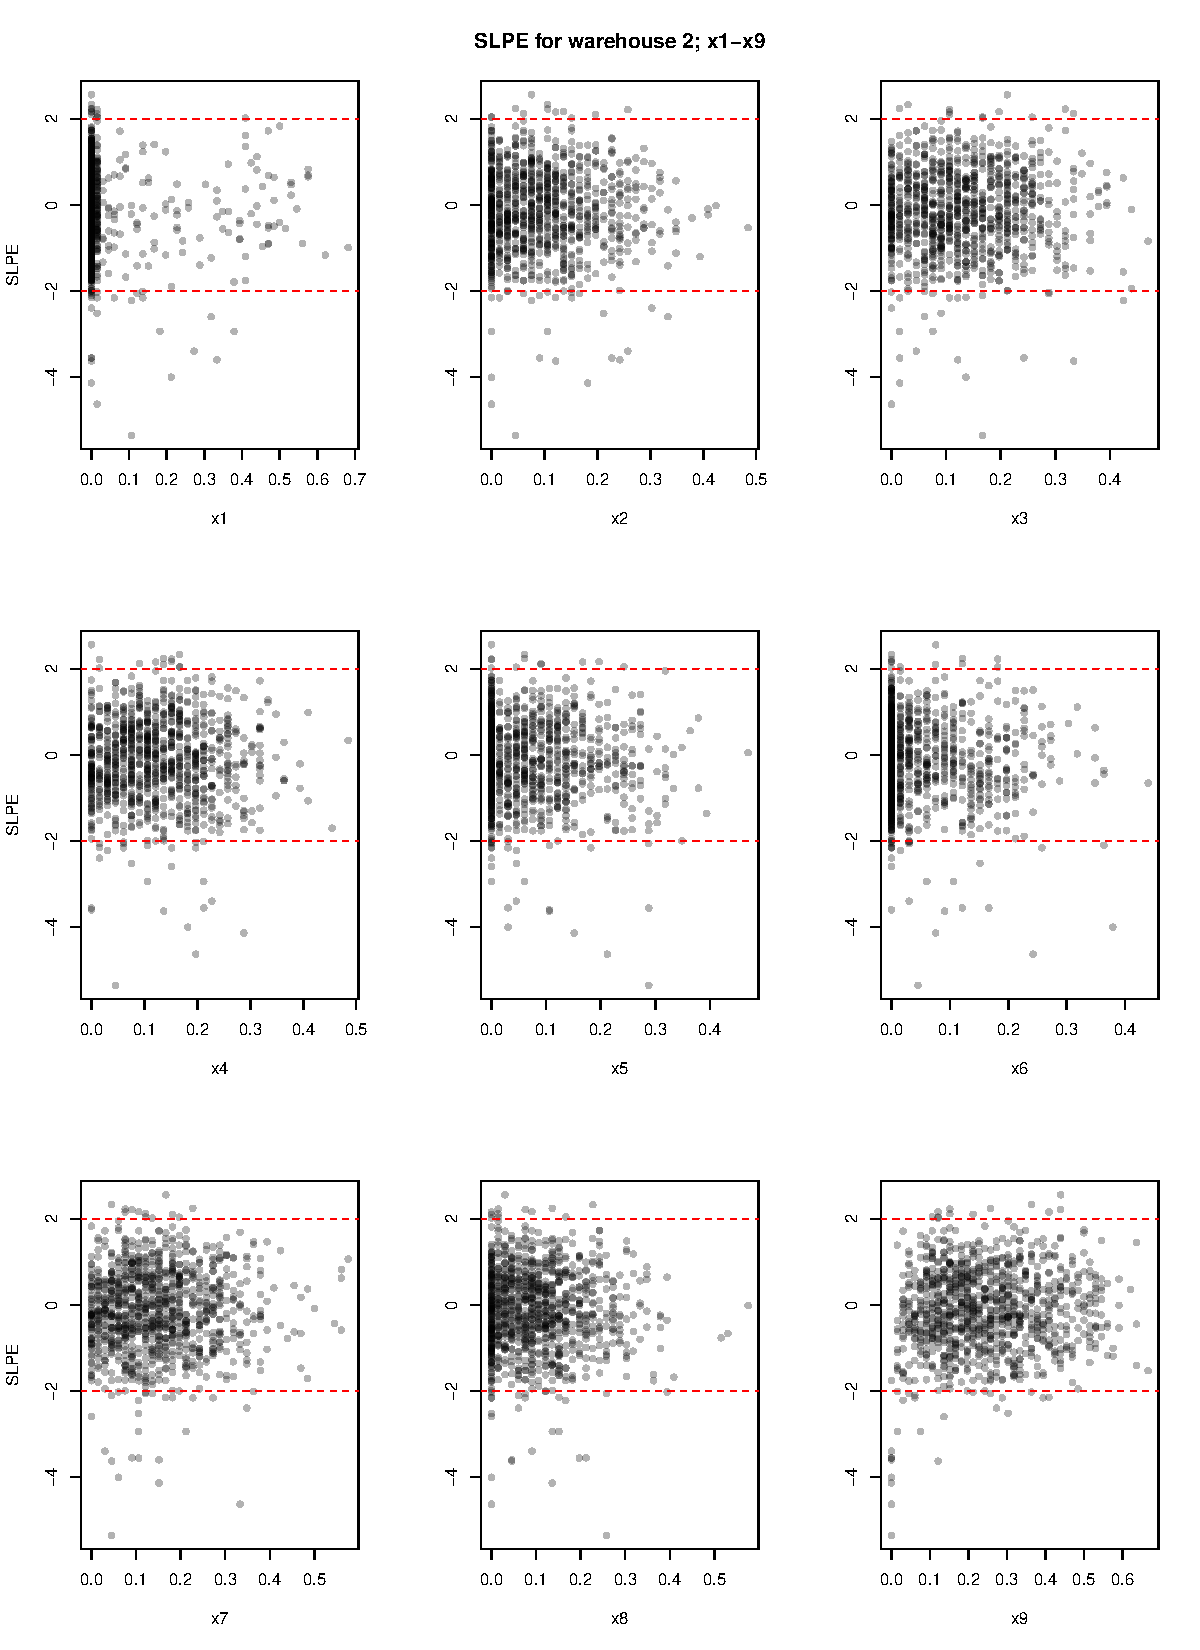
\includegraphics[width=\textwidth]{fig-app-ds/w1-w2-1.pdf}
  \caption{SLPEs for the first $9$ inputs of the wave $1$ emulator, for warehouse $2$ and $h(\bx) = 1$.}
\end{figure}

\begin{figure}
  \centering
  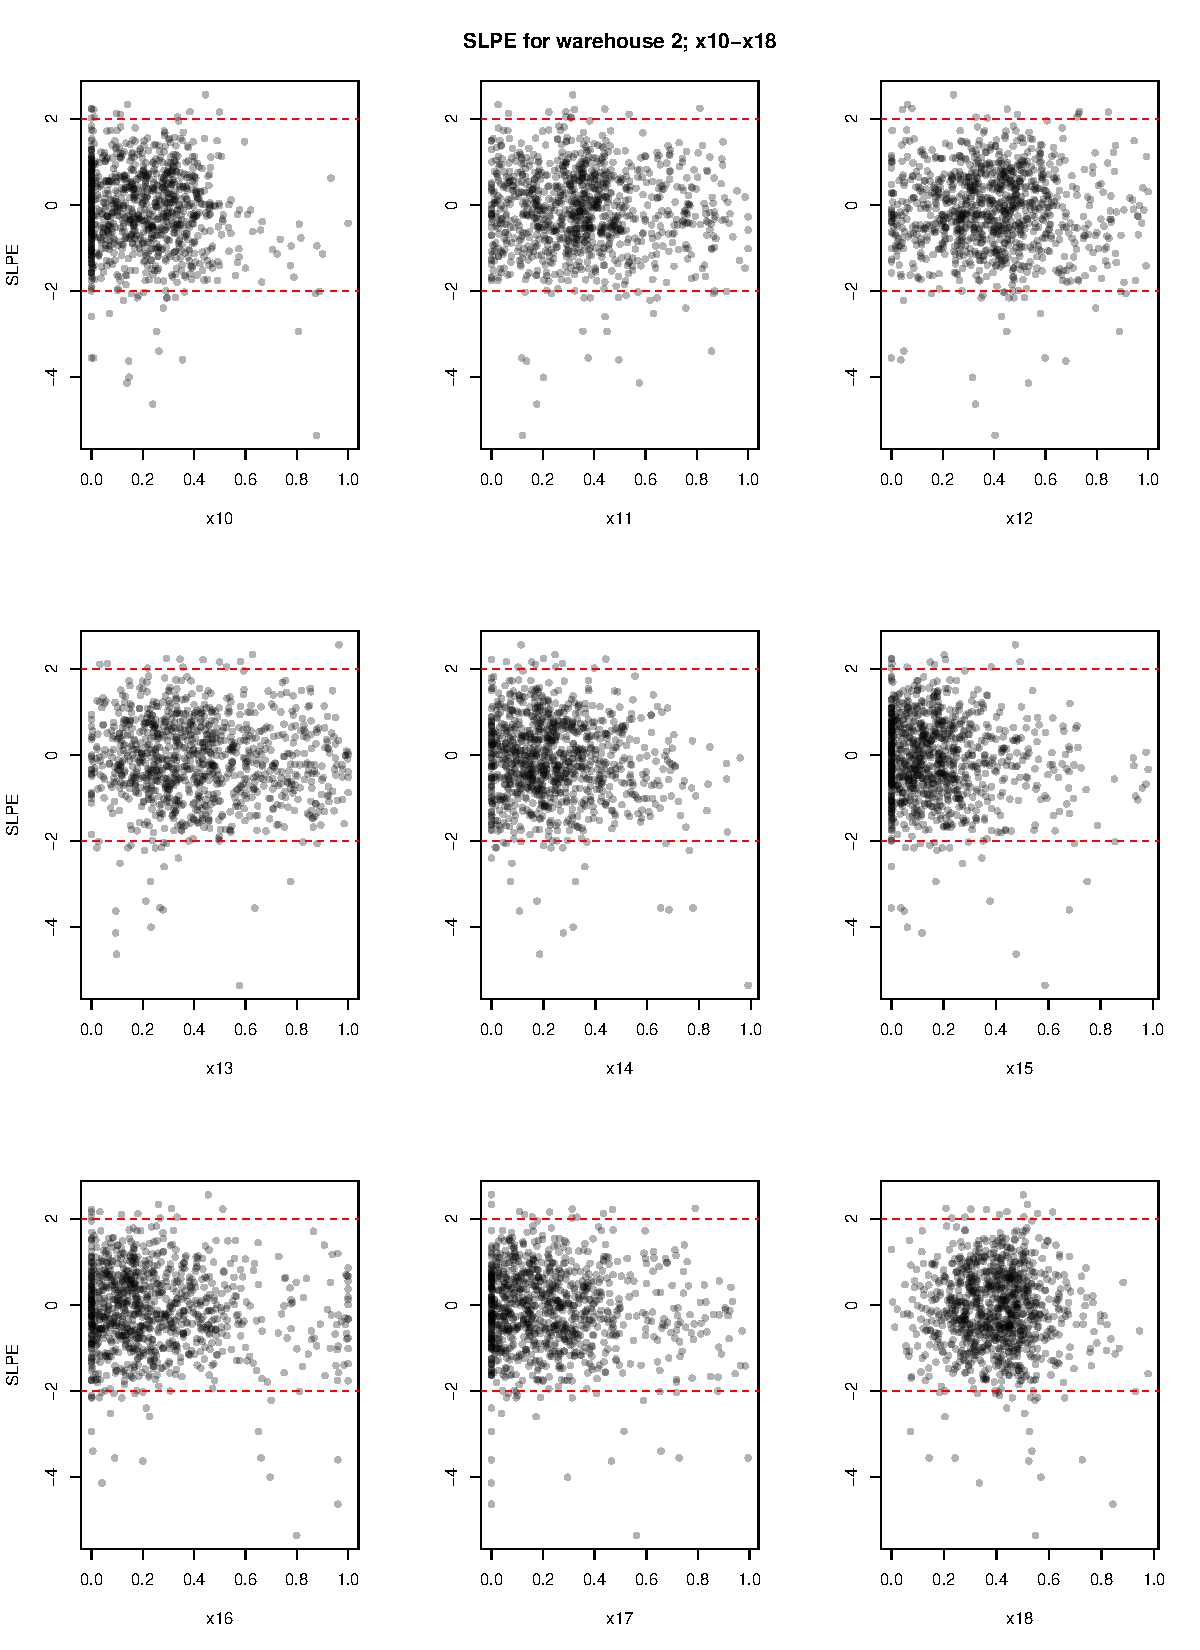
\includegraphics[width=\textwidth]{fig-app-ds/w1-w2-2.pdf}
  \caption{SLPEs for the last $9$ inputs of the wave $1$ emulator, for warehouse $2$ and $h(\bx) = 1$.}
\end{figure}
%wave 1, warehouse 3, no mean
\begin{figure}
  \centering
  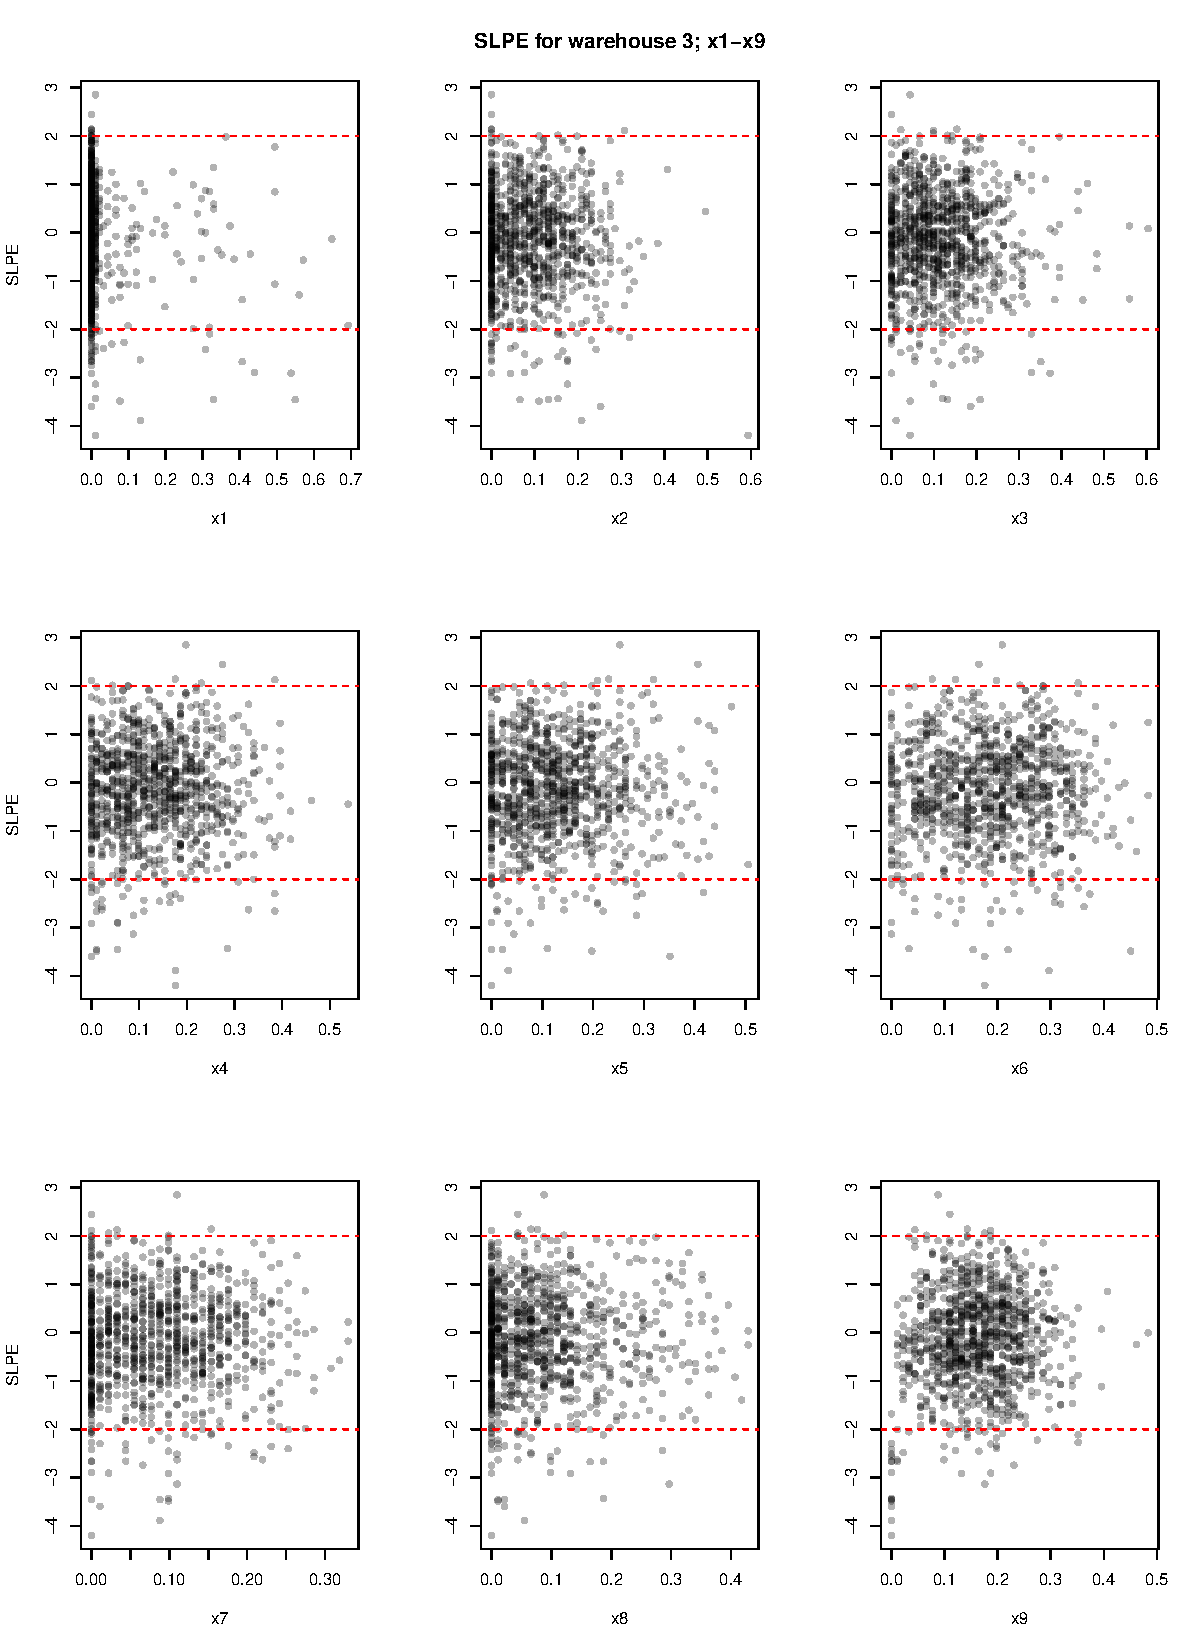
\includegraphics[width=\textwidth]{fig-app-ds/w1-w3-1.pdf}
  \caption{SLPEs for the first $9$ inputs of the wave $1$ emulator, for warehouse $3$ and $h(\bx) = 1$.}
\end{figure}

\begin{figure}
  \centering
  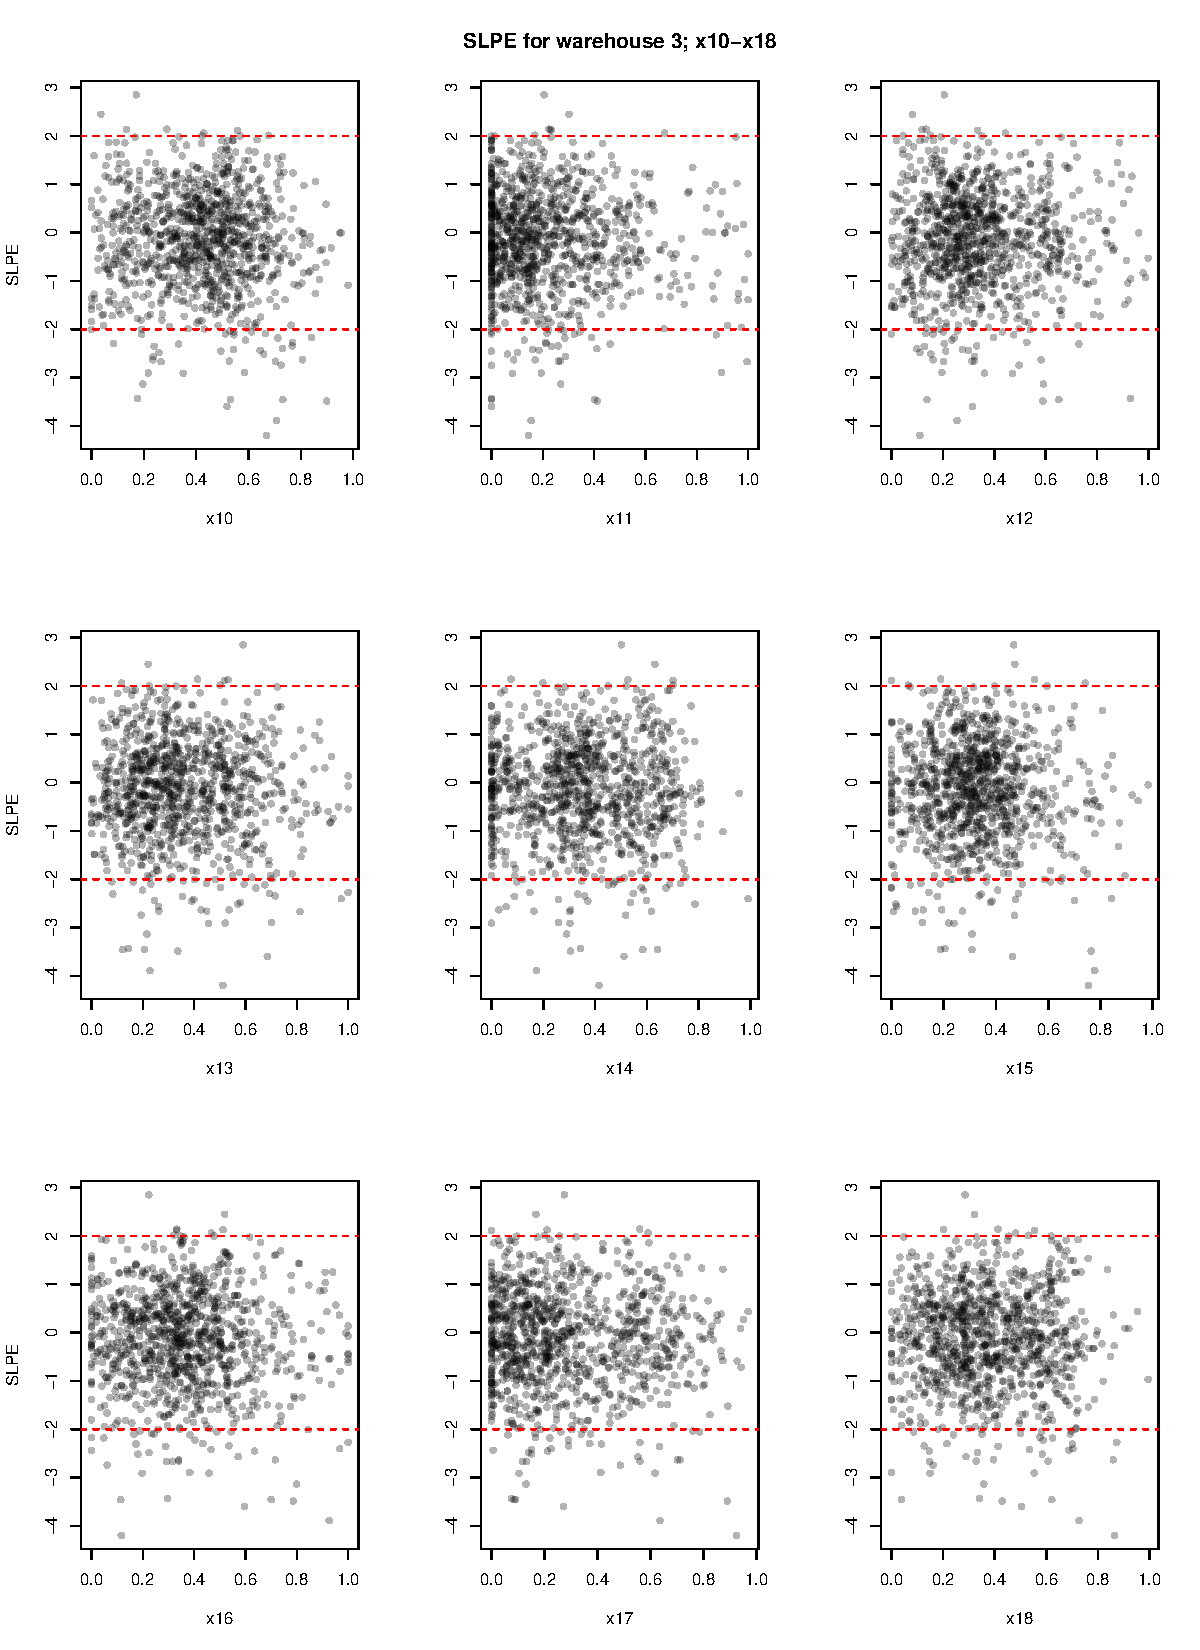
\includegraphics[width=\textwidth]{fig-app-ds/w1-w3-2.pdf}
  \caption{SLPEs for the last $9$ inputs of the wave $1$ emulator, for warehouse $3$ and $h(\bx) = 1$.}
\end{figure}
\newpage
\section{Plots of SLPEs for the wave $1$ emulator, with mean function \label{App:resid2}}
The following $6$ plots correspond directly to the previous $6$. In particular, the values on the $x$ axis are exactly the same in the corresponding plots. The change here is that the residuals are from a different emulator; in particular, the mean function is $h(\bx) = (1, \log (x_9 + 10^{-8})$ and the prior $\beta_i \iid \mathcal{N}\{0, 0.5^2 \}$ is assigned to the regression parameters (but integrated out to allow for efficient computation).
%wave 1, warehouse 1, with mean
\begin{figure}
  \centering
  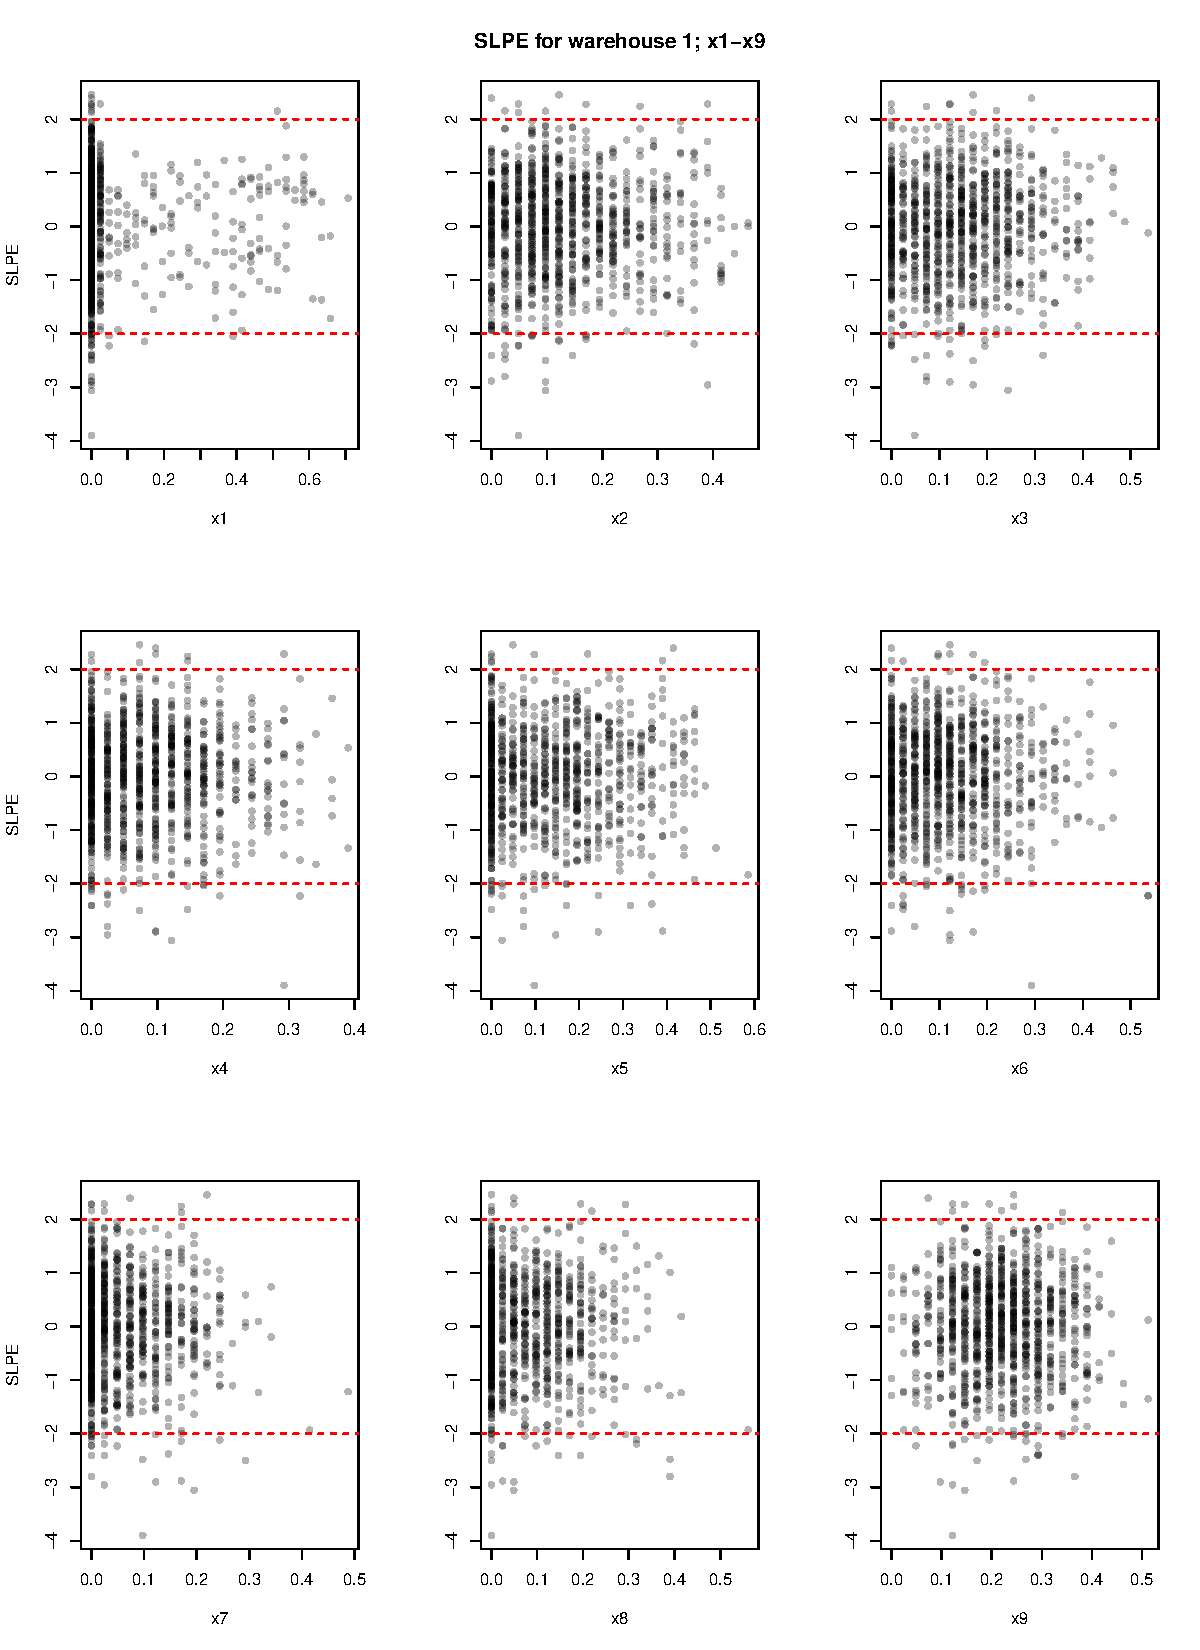
\includegraphics[width=\textwidth]{fig-app-ds/w1-w1-mean1.pdf}
  \caption{SLPEs for the first $9$ inputs of the wave $1$ emulator, for warehouse $1$ and $h(\bx) = (1, \log (x_9 + 10^{-8}))$.}
\end{figure}

\begin{figure}
  \centering
  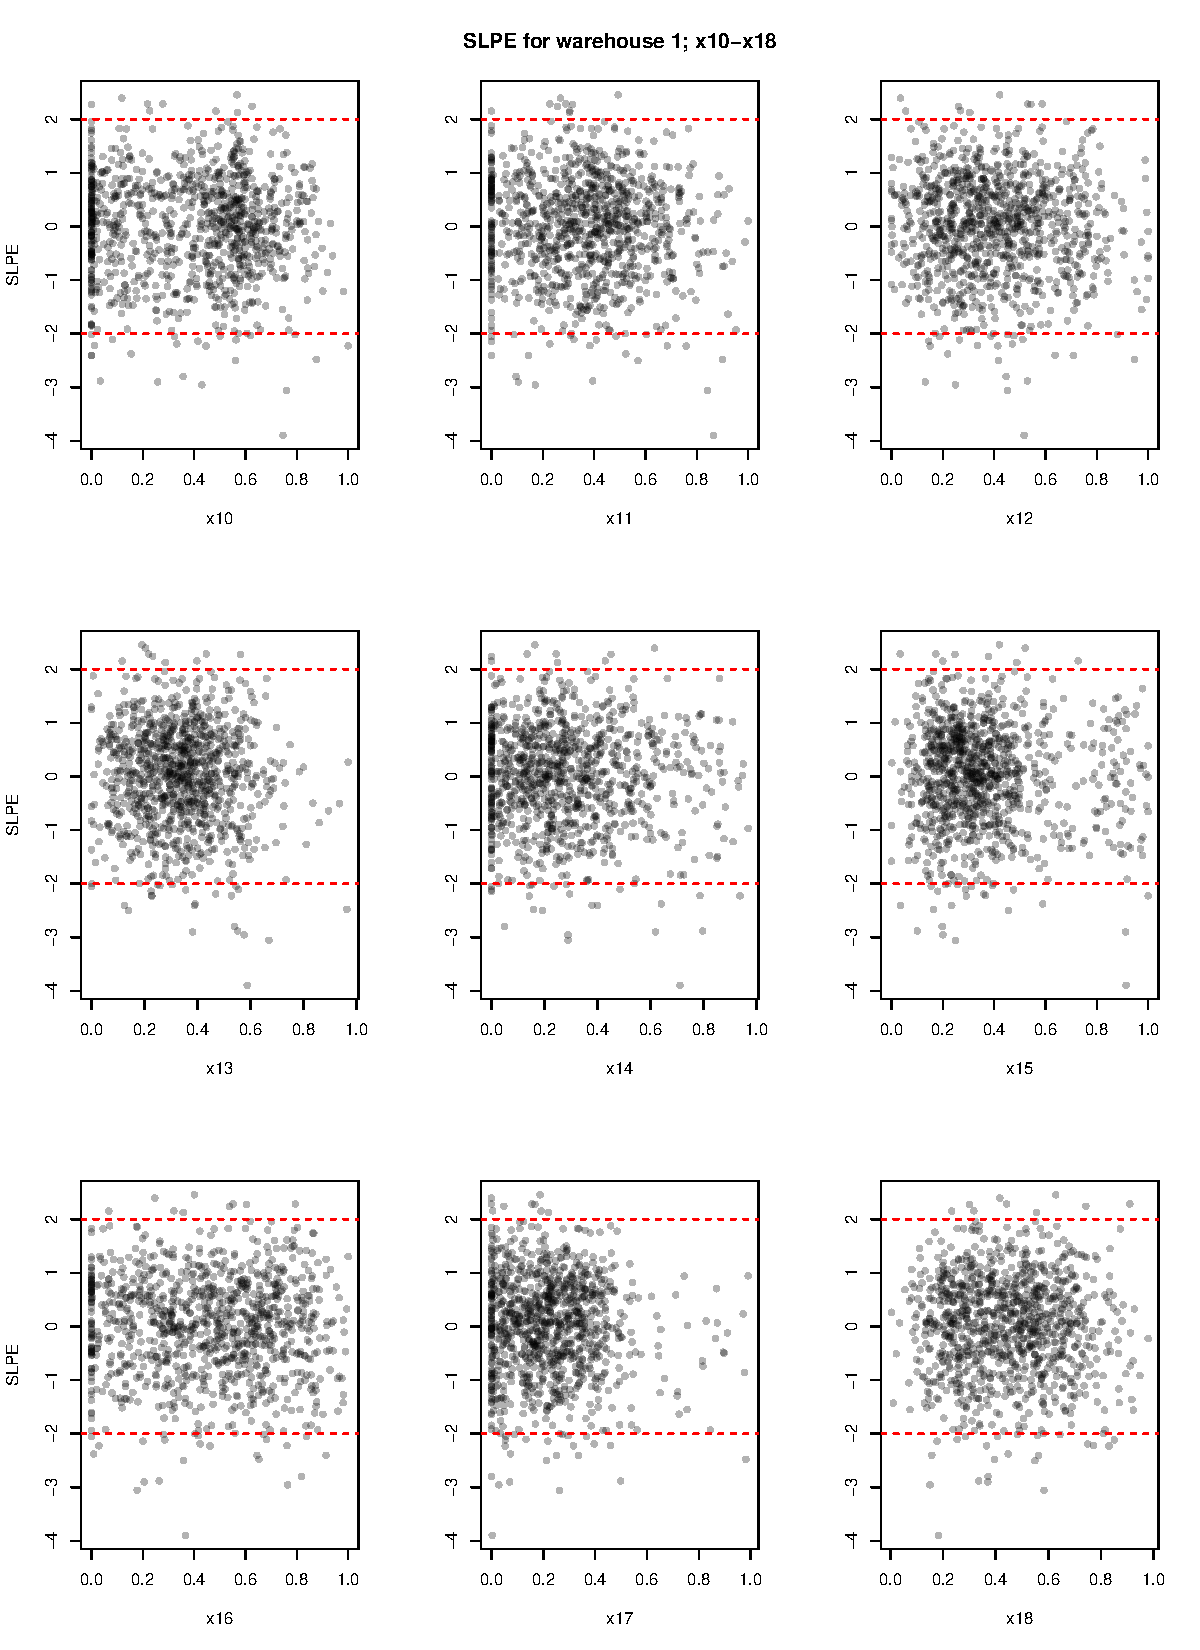
\includegraphics[width=\textwidth]{fig-app-ds/w1-w1-mean2.pdf}
  \caption{SLPEs for the last $9$ inputs of the wave $1$ emulator, for warehouse $1$ and $h(\bx) = (1, \log (x_9 + 10^{-8}))$.}
\end{figure}
%wave 1, warehouse 2, with mean
\begin{figure}
  \centering
  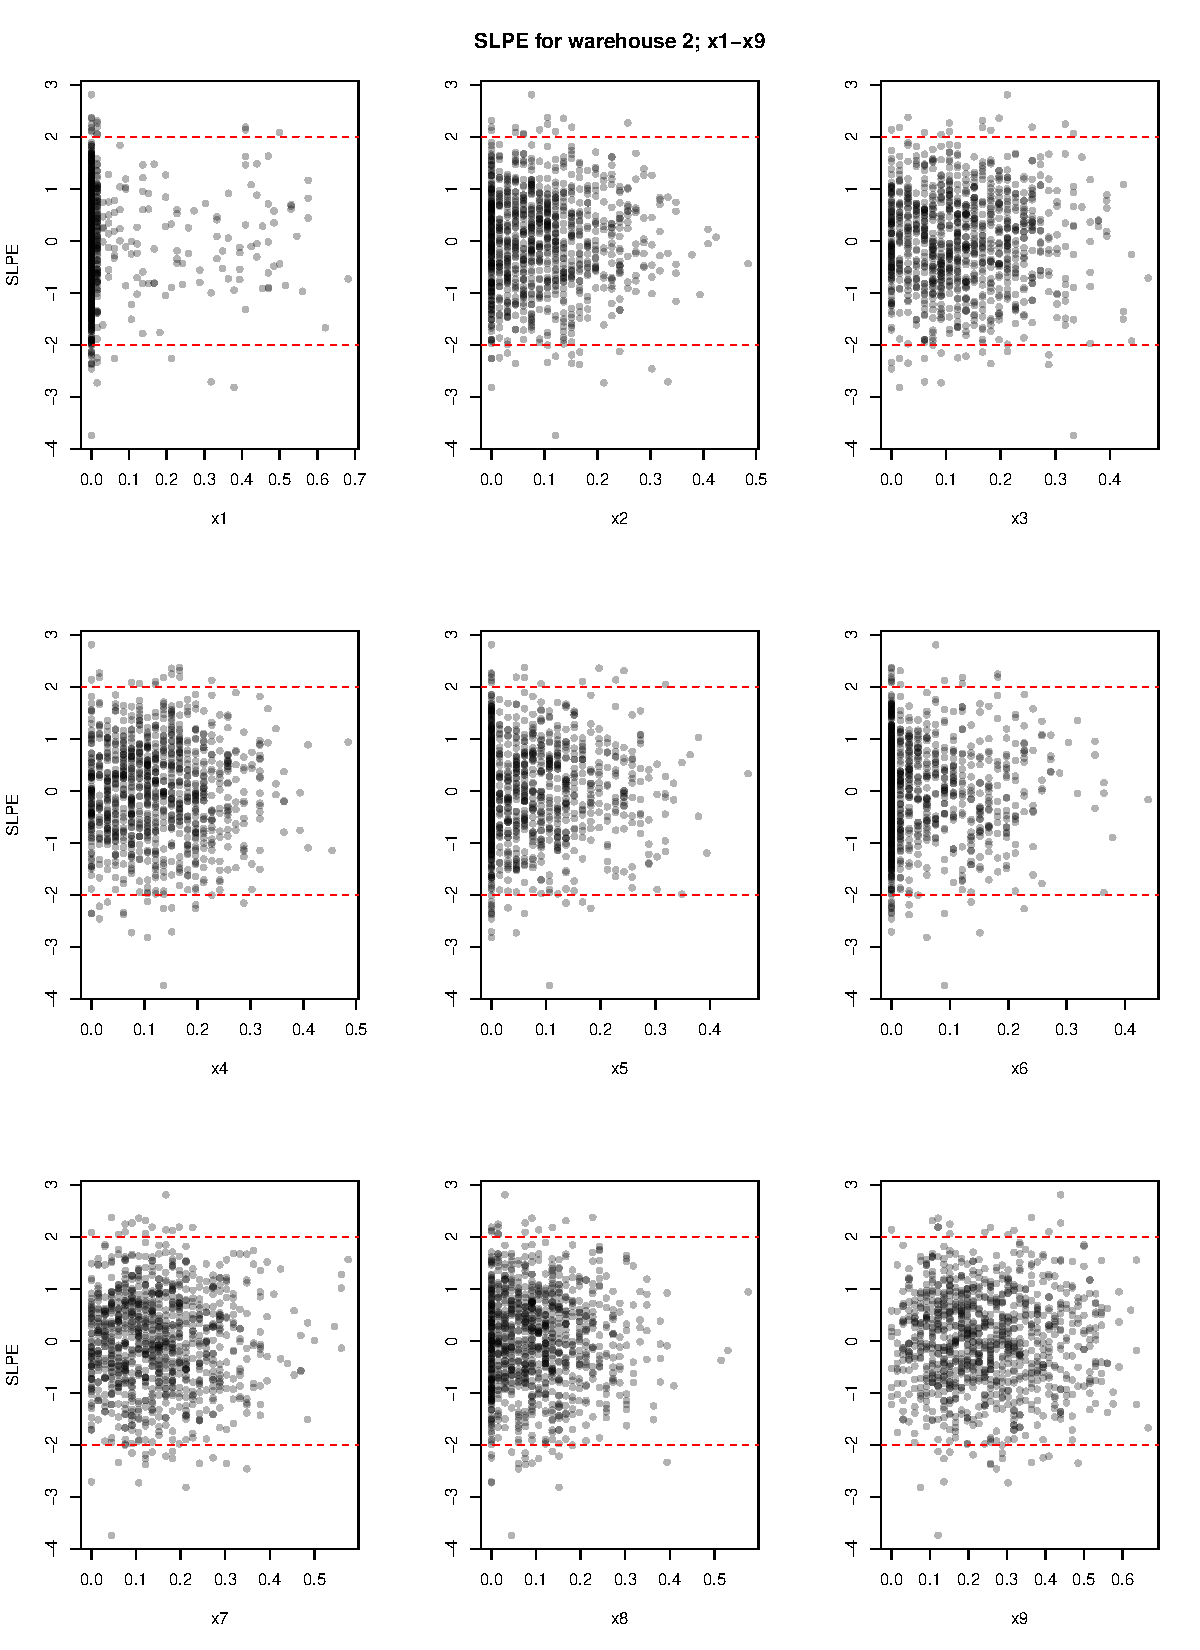
\includegraphics[width=\textwidth]{fig-app-ds/w1-w2-mean1.pdf}
  \caption{SLPEs for the first $9$ inputs of the wave $1$ emulator, for warehouse $2$ and $h(\bx) = (1, \log (x_9 + 10^{-8}))$.}
\end{figure}

\begin{figure}
  \centering
  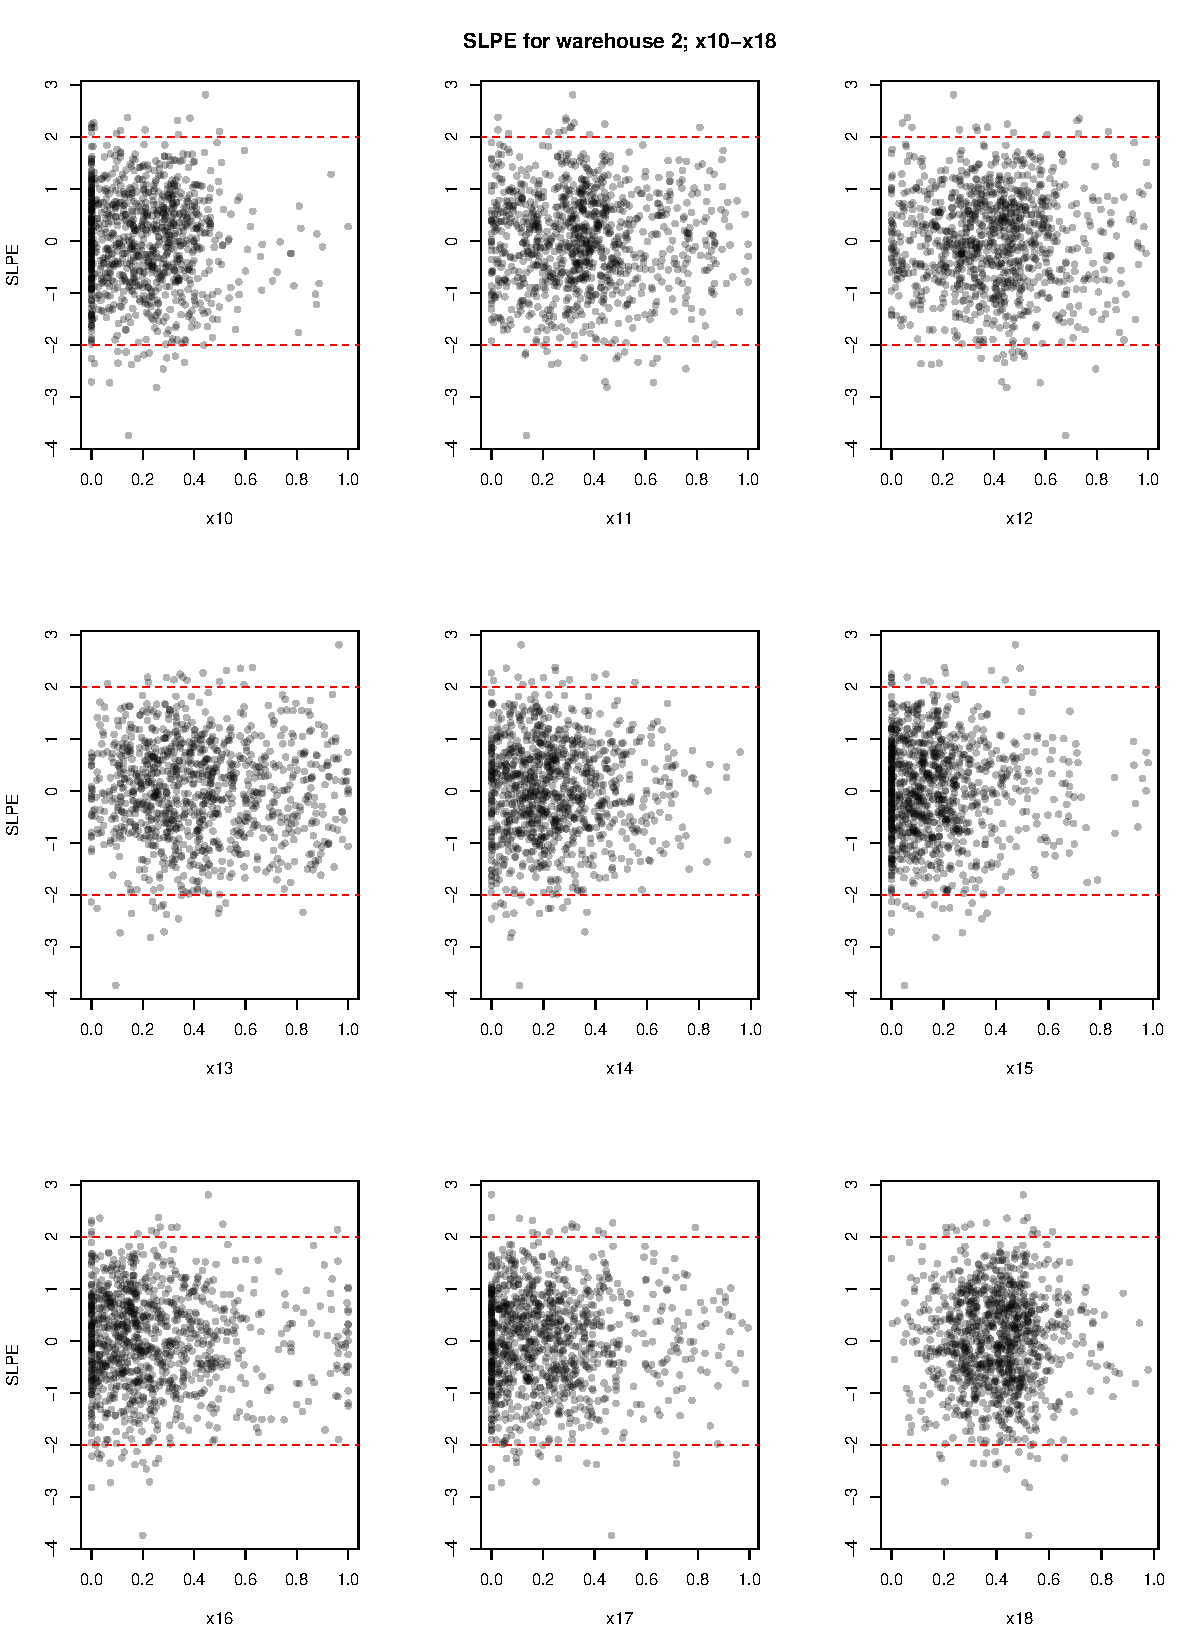
\includegraphics[width=\textwidth]{fig-app-ds/w1-w2-mean2.pdf}
  \caption{SLPEs for the first $9$ inputs of the wave $2$ emulator, for warehouse $2$ and $h(\bx) = (1, \log (x_9 + 10^{-8}))$.}
\end{figure}
%wave 1, warehouse 3, with mean
\begin{figure}
  \centering
  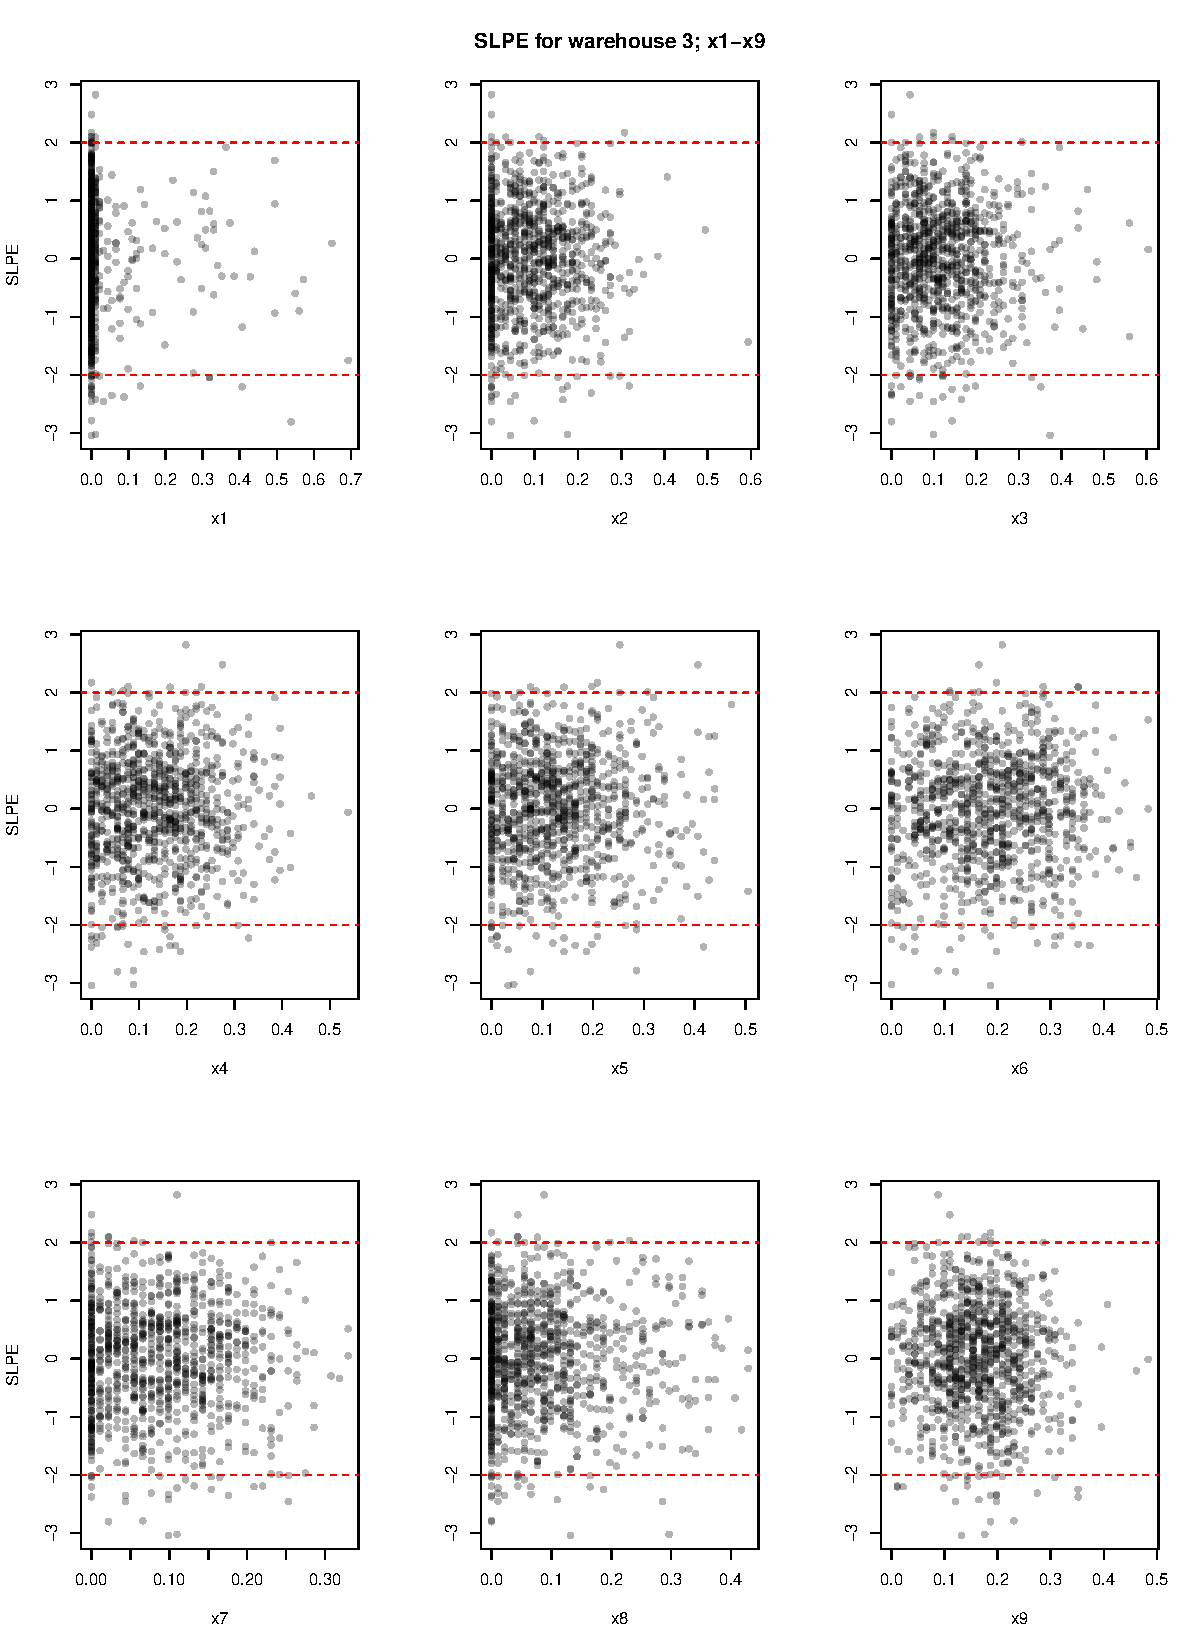
\includegraphics[width=\textwidth]{fig-app-ds/w1-w3-mean1.pdf}
  \caption{SLPEs for the first $9$ inputs of the wave $1$ emulator, for warehouse $3$ and $h(\bx) = (1, \log (x_9 + 10^{-8}))$.}
\end{figure}

\begin{figure}
  \centering
  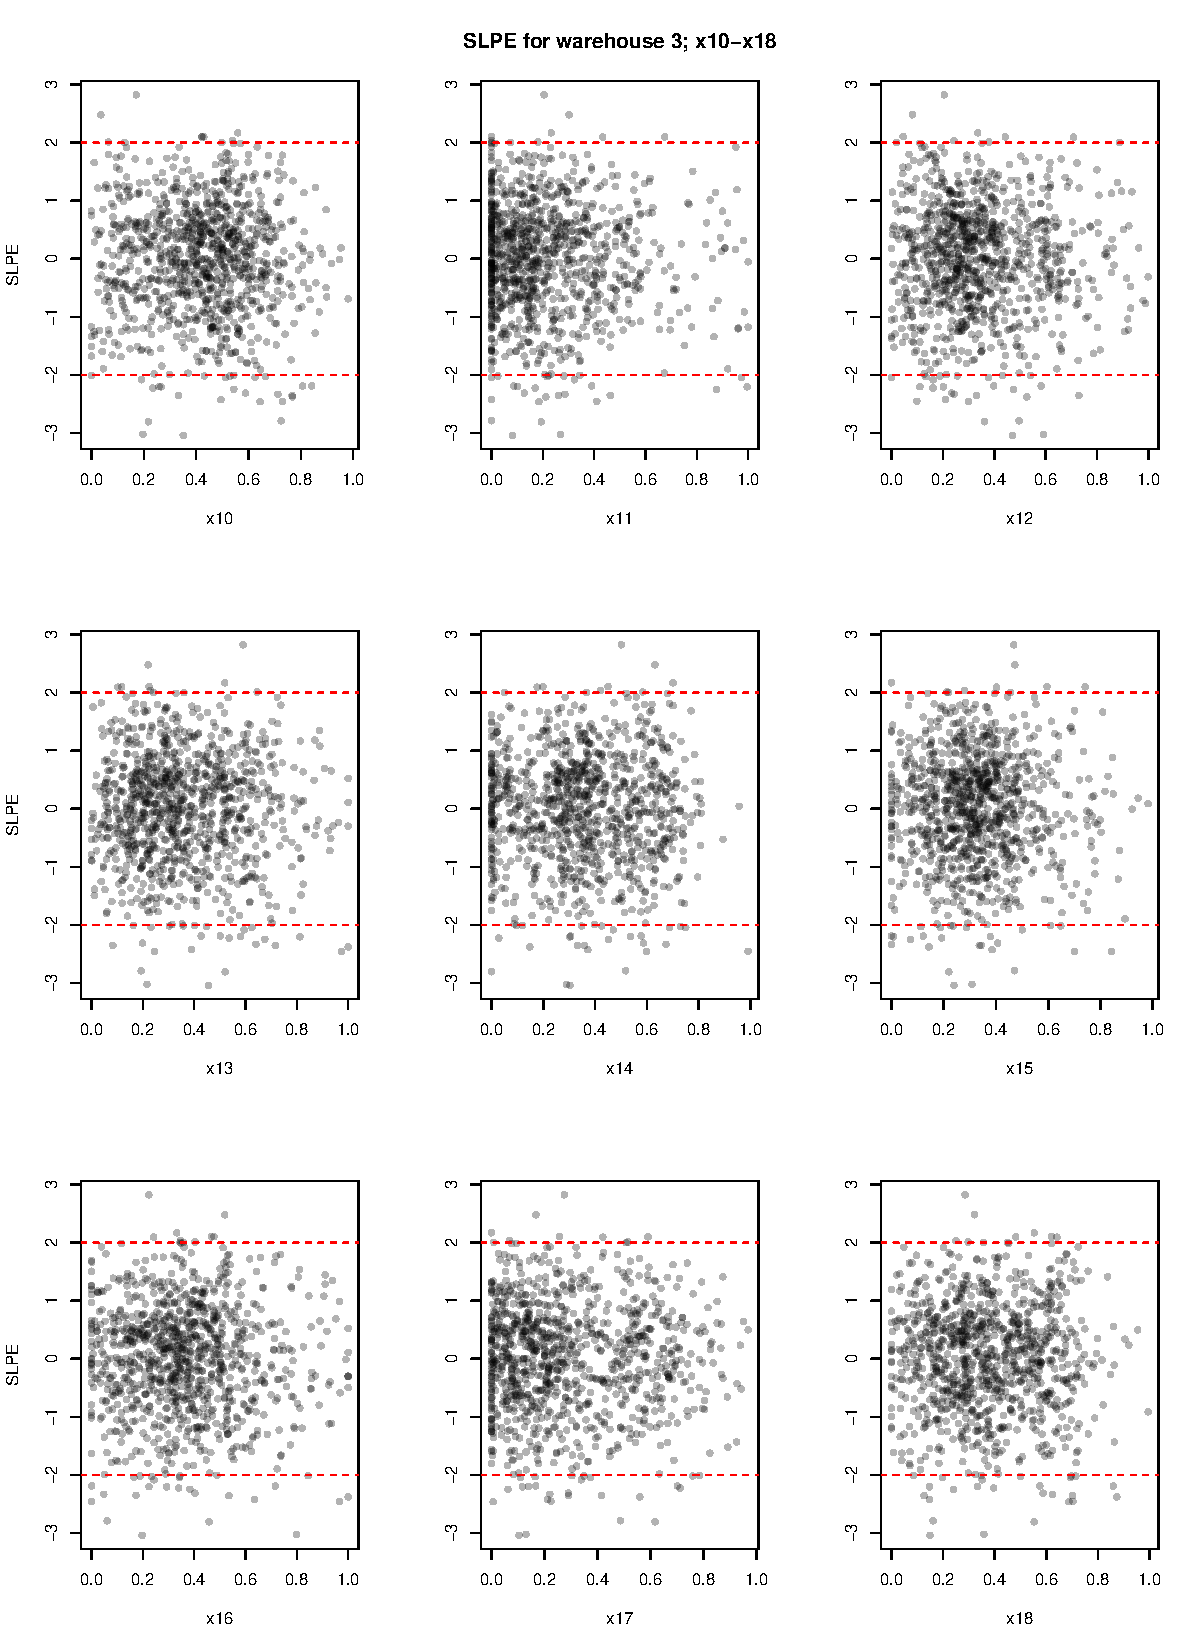
\includegraphics[width=\textwidth]{fig-app-ds/w1-w3-mean2.pdf}
  \caption{SLPEs for the last $9$ inputs of the wave $1$ emulator, for warehouse $3$ and $h(\bx) = (1, \log (x_9 + 10^{-8}))$.}
\end{figure}
\newpage
\section{Plots of SLPEs for the wave $2$ emulators \label{App:resid3}}
The following plots show the SLPEs plotted against the inputs for the wave $2$ emulators. Since warehouse $3$ was dropped from  the analysis, this section has only $4$ plots (a pair for warehouse $1$, a pair for warehouse $2$).

Some of the plots show a slight pattern, however, improving the complexity of the mean function \textit{did not} improve the fit. We put this down the the asymmetry in the distribution of $y(\bx)$, which is present in \cref{Fig:bootstrap}. In particular, the asymmetry in the residual plots below matches the general pattern of the bootstrap distributions in \cref{Fig:bootstrap}; all the plots indicate (mild) left-skew.
\begin{figure}
  \centering
  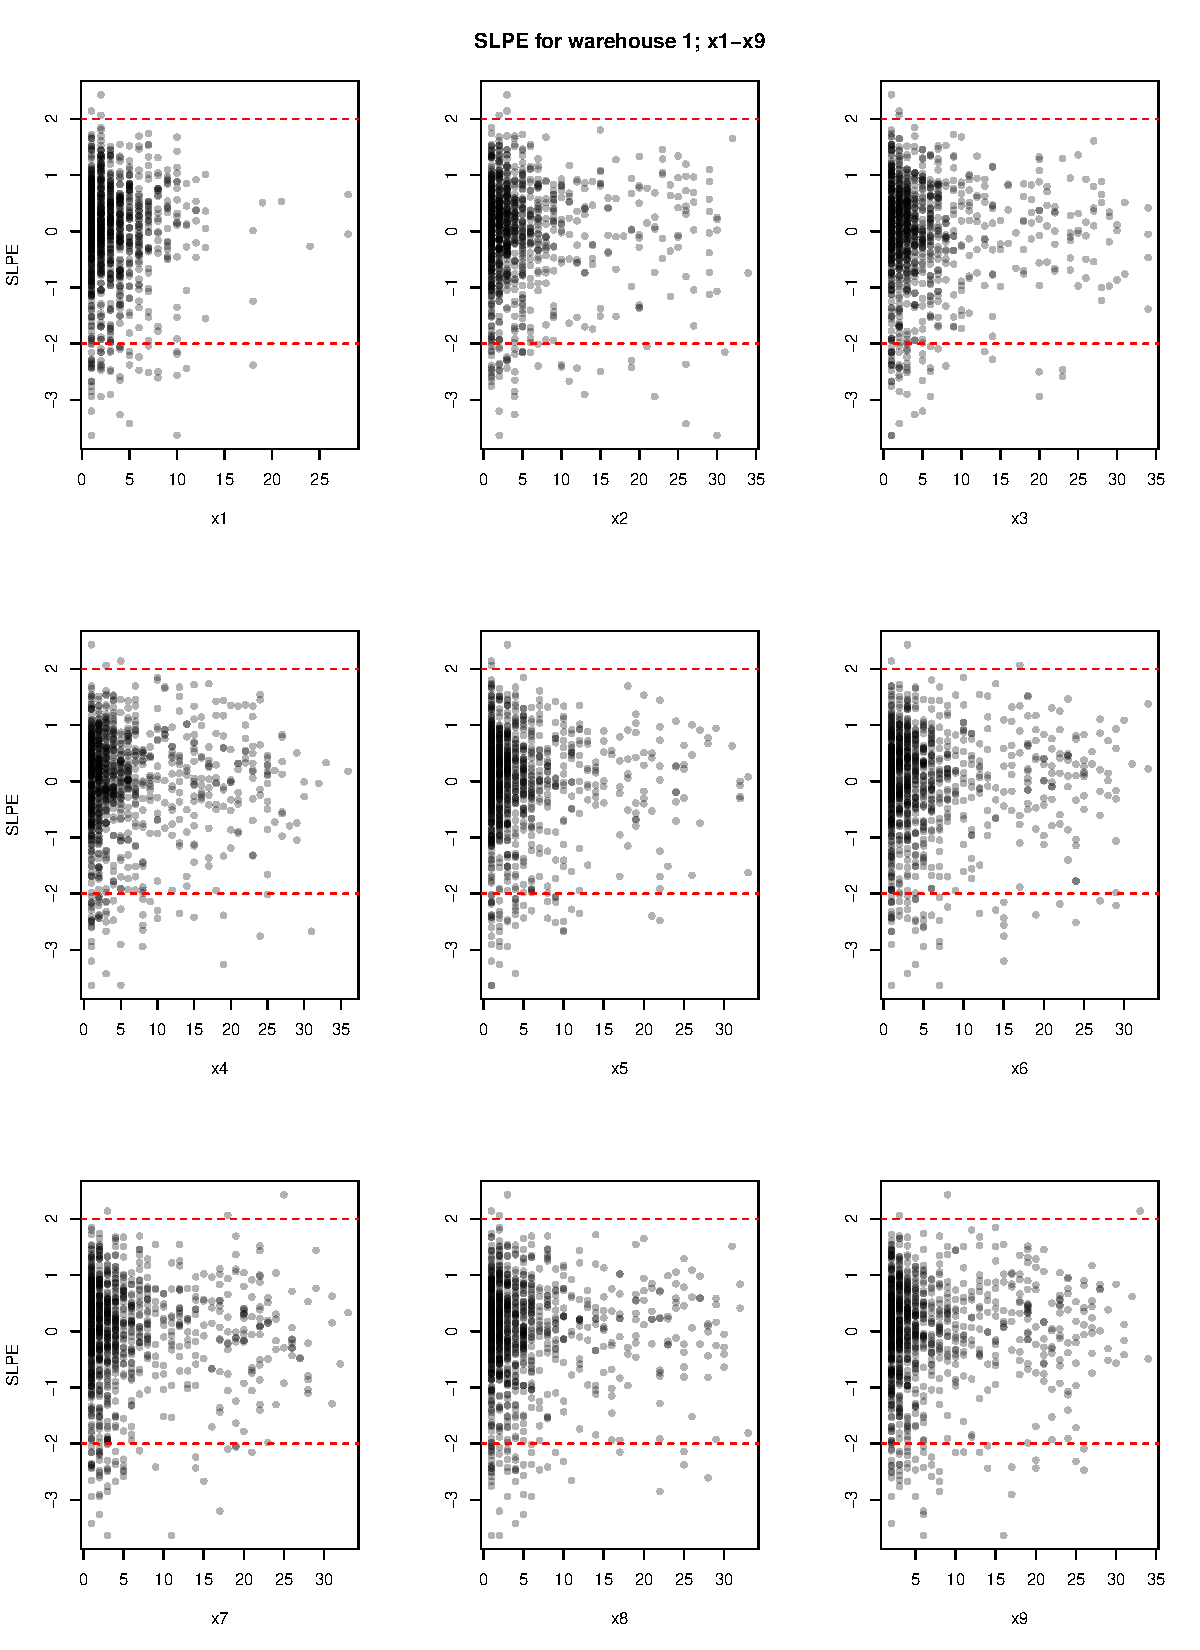
\includegraphics[width=\textwidth]{fig-app-ds/w2-w1-1.pdf}
  \caption{SLPEs for the first $9$ inputs of the warehouse $1$, wave $2$ emulator.}
\end{figure}

\begin{figure}
  \centering
  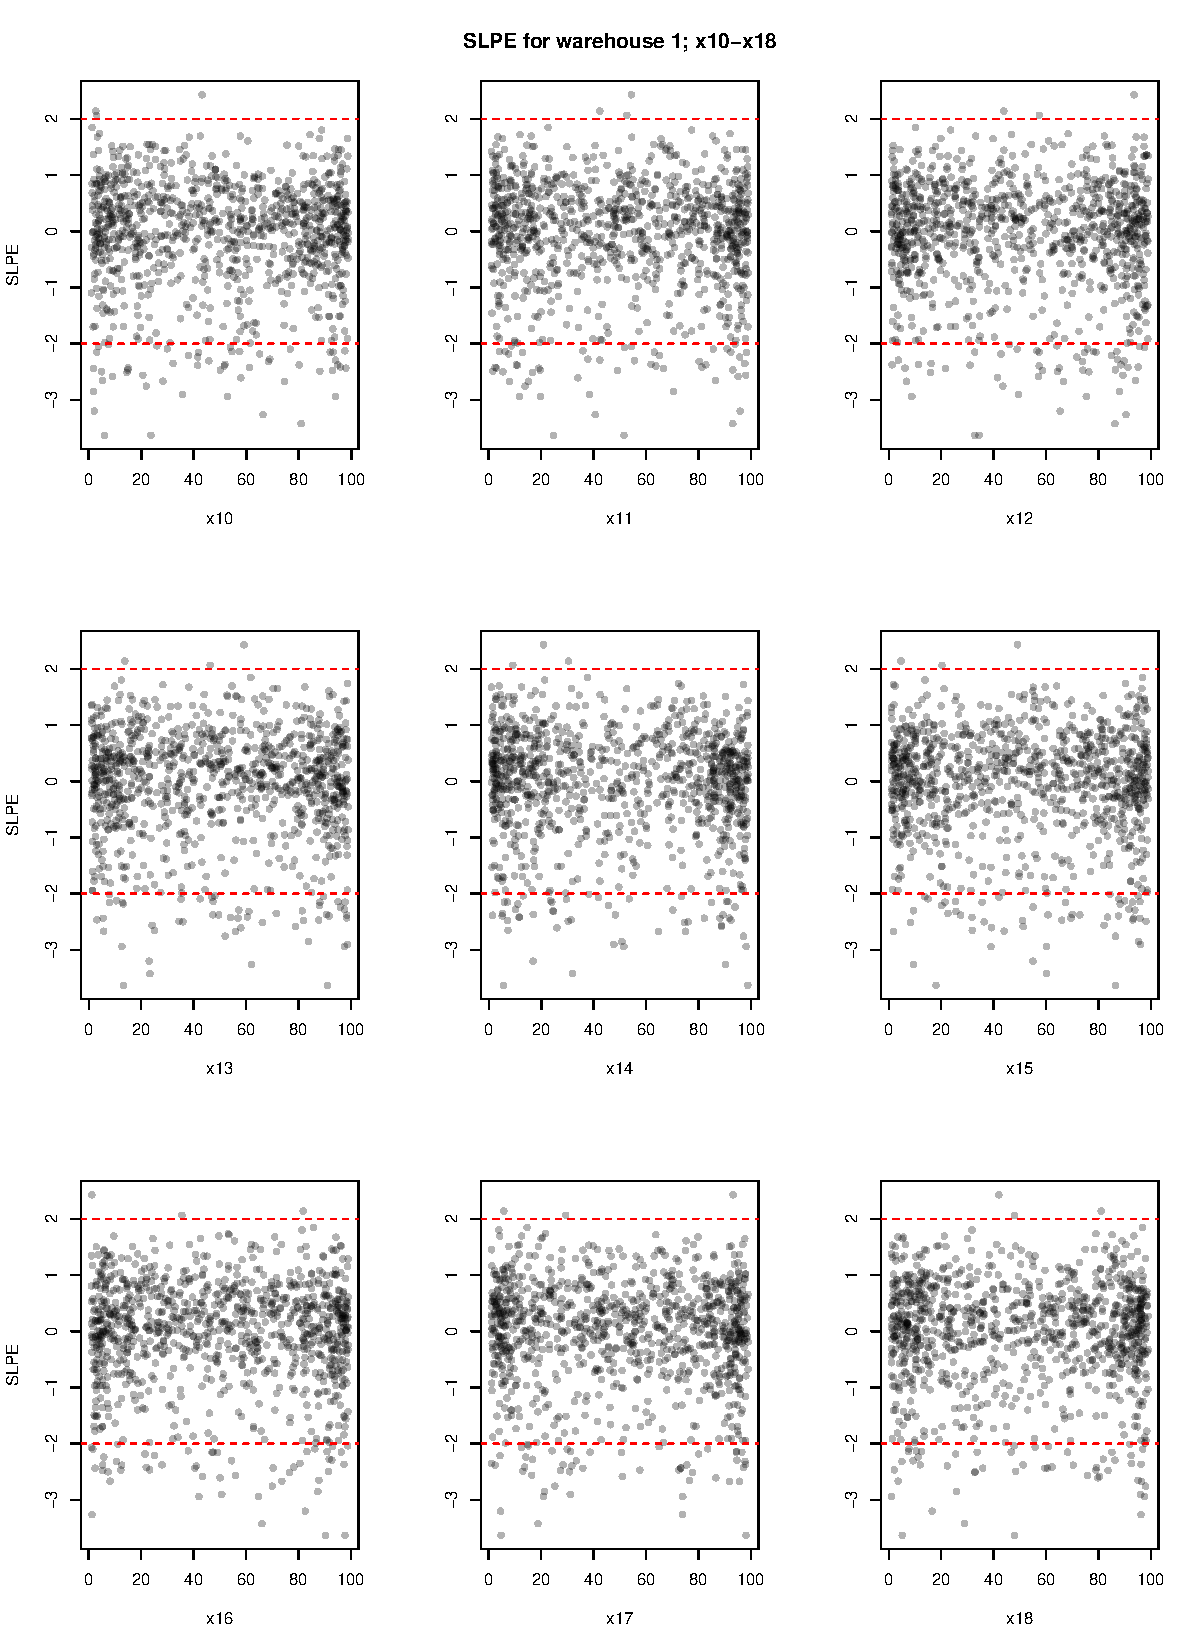
\includegraphics[width=\textwidth]{fig-app-ds/w2-w1-2.pdf}
  \caption{SLPEs for the last $9$ inputs of the warehouse $1$, wave $2$ emulator.}
\end{figure}
%wave 1, warehouse 2, with mean
\begin{figure}
  \centering
  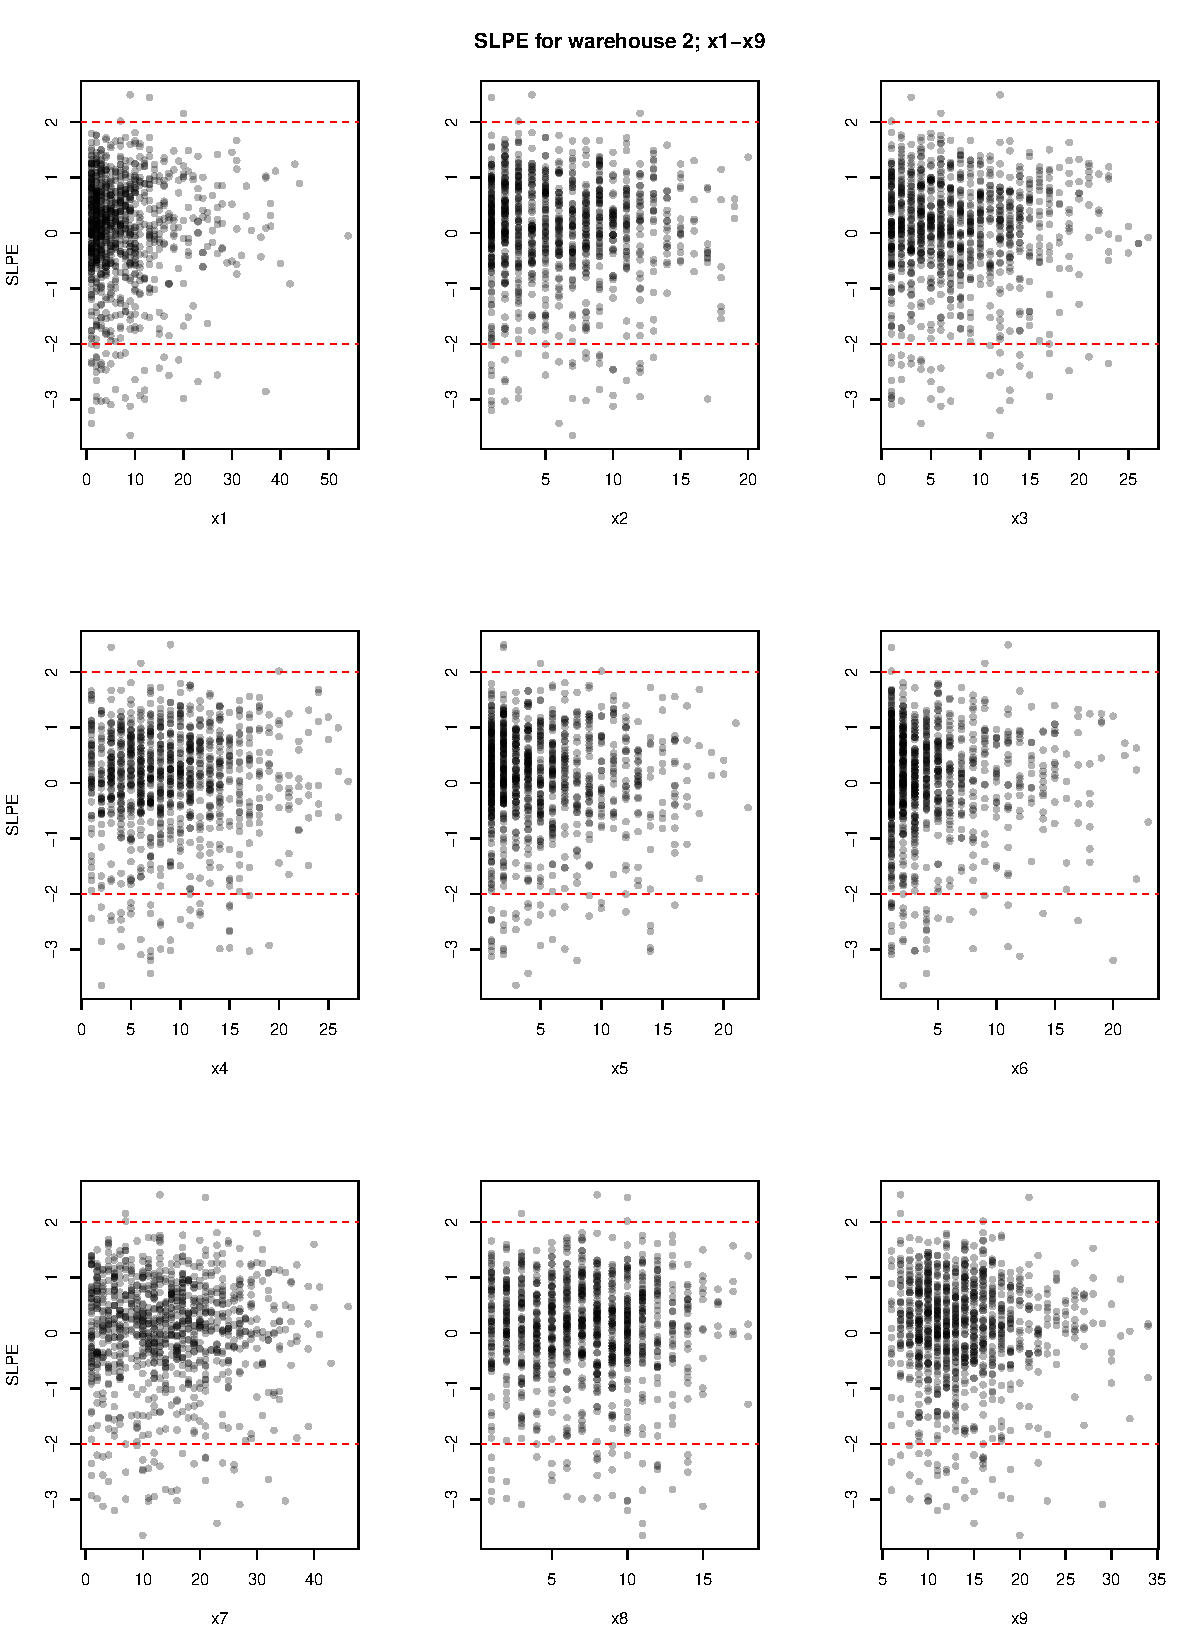
\includegraphics[width=\textwidth]{fig-app-ds/w2-w2-1.pdf}
  \caption{SLPEs for the first $9$ inputs of the warehouse $2$, wave $2$ emulator.}
\end{figure}

\begin{figure}
  \centering
  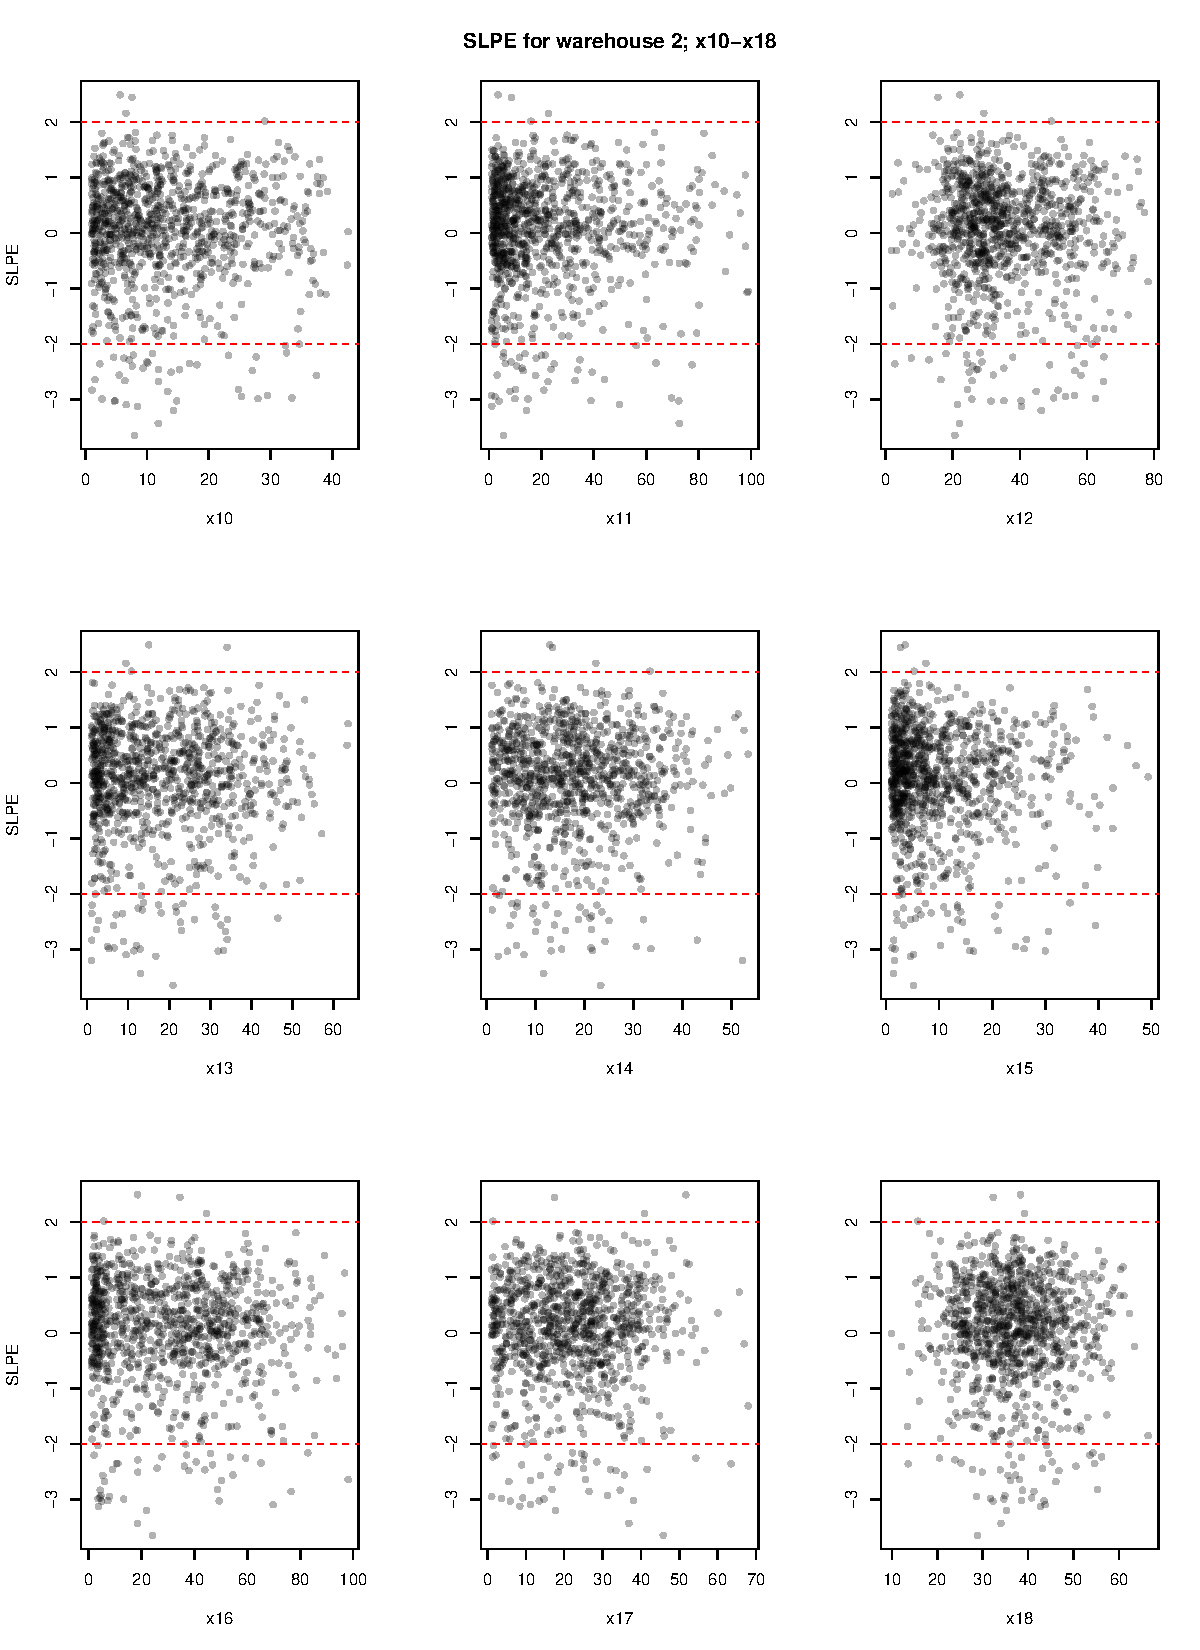
\includegraphics[width=\textwidth]{fig-app-ds/w2-w2-2.pdf}
  \caption{SLPEs for the first $9$ inputs of the warehouse $2$, wave $2$ emulator.}
\end{figure}
\end{chapter}
